\section{Experiments}

In this section we provide results on modeling ablation studies, online A/B experiments with OON application and infrastructure model-based retrieval inference benchmarking for production indexes.

\subsection{Model offline evaluation}\label{sec:offline_evaluation}
We evaluated {\systemname} model on our internal dataset. The dataset consists of millions of examples where a member interacted with an item. The member and item are represented by embeddings learnt from a two-tower model.
The two-tower model contains variety of features including member interaction history modeled by \cite{nxtpost_paper} and member profile features, which usually contains member job title, job location, company, skills and professional summary of the member. Posts usually contain text, image, video or external link information. Therefore, such content features from member and posts can help us to identify topics of interests of posts or professional topics of members. 

\begin{comment}
A mixture inherently requires us to have multiple features.
We augmented our data with the following methods:
\begin{itemize}
\item \textbf{k-means++}:
Given embeddings of members and posts in the same space, we cluster them using k-means++ in offline and store cluster centers as part of the {\systemname} model.
\item \textbf{Learnt clustering}:
We learn soft clusters from the engagement data. We take top $K$ clusters. The clusters represent engagement patterns of those topics. Cluster embeddings could be initialized randomly or with offline kmeans centroid values. 
\item \textbf{Residual Id embeddings}:
We learn id embeddings for popular members and posts and sum them together in the model with clusterID embeddings in residual manner for more robust feature representation. The id embeddings are randomly initialized closely to zero.
\end{itemize}

The best model applies all combinations of distances \{Hadamard, Weighted Cosine\} to provided embedding components \{k-means++, Learnt clustering, Residual Id\} referred in the Table \ref{table:mix_of_similarities} as \textit{Mixture of Similarities with feature augmentation}. It means that every learnt distance function is applied to every embedding combination.
\end{comment}

%% mizhou: removed table for cluster activation function
% \begin{table}[ht]
% % centering
% \small % This command makes the text of the table smaller
% \vspace{-4pt}
% \begin{tabular}{lcc}
% \hline
% \textbf{Method}
% & \textbf{Gain in Hit Rate @ 100} \\\hline 
% Cosine similarity with exhaustive scan & -  \\
% % Weighted inner product & 0.00117 \\
% % Hadamard MLP  & 0.00113 \\
% MoL with learnt clusterID (sigmoid) & -9.66\%  \\
% \textbf{MoL with learnt clusterID (relu)}  & \textbf{8.56\%} \\\hline
% \end{tabular}
% \caption{Evaluation of Mixture-of-Logits on industrial dataset}
% \label{table:mix_of_similarities}
% \vspace{-12pt}
% \end{table}

%As part of the MoL we generated several projections of the original two tower embeddings, we used 4 projections for member and 8 projections for the item, generating 32 combinations of distances. We sum up clusterID embeddings with all of projection of the two tower item embeddings resulting in 32 components of MoL.
We used Hit Rate @ 400 over evaluation dataset to report the metrics. We use cosine similarity with exhaustive search as baseline to evaluate against {\systemname}. We report results of Hadamard MLP for single embedding feature and extended Mixture-of-Logits with clustering for both single and multi-embedding features in Table \ref{table:offline_eval}.

Hadamard MLP is favored for production due to its simplicity for deployment and low latency. However, we found Hadamard MLP is very sensitive to weight initialization and general initialization methods such as GlorotNormal or HeNormal can't stabilize the performance. Empirically we observed that the initial few steps determine the overall training trend, Thus we reinitialize the model if the first 100 steps go south.

In addition to the two-tower model and cluster ID features, we enhanced Mixture-of-Logits by introducing multiple embedding features developed at LinkedIn. We incorporated Graph Neural Network (GNN) embeddings for members and posts mapped to the same space using a heterogeneous GNN~\cite{borisyuk2024lignn}. We found that adding more embeddings improved the Hit Rate @ 400 (see Table \ref{table:offline_eval}).

Our extended Mixture-of-Logits with clustering perform well for both single and multi-embedding features. One surprise finding is that fixed clusters (non-trainble) outperform trainable clusters in all cases we explored, one possible explanation is the convergence pace of the clustering and other trainable parameters are different, we'll further investigate it in our future work. Another interesting observation is that it was important to carefully tune the number of clusters: having either too high or too low a value can cause performance to degrade.
\begin{table}[ht]
% centering
\small % This command makes the text of the table smaller
\vspace{-4pt}
\begin{tabular}{lcc}
\hline
\textbf{Method}
& \textbf{Gain in Hit Rate @ 400} \\\hline 
Cosine similarity & --  \\\hline
\textbf{Single Embedding Feature} \\ %\hline
Hadamard(Member \& Item MLP [50]+[10, 1]) & 10.21\% \\
MoL with 70 trained | non-trained clusters & 1.33\% | 10.11\% \\
MoL with 100 trained | non-trained clusters & 11.97\% | \textbf{15.16\%} \\
MoL with 150 trained | non-trained clusters & 4.26\% | 11.17\% \\\hline
\textbf{Multiple Embedding Features} \\ %\hline
MoL without clustering & 12.80\% \\
MoL with 140 trained | non-trained clusters & 20.75\% | 22.61\% \\
MoL with 200 trained | non-trained clusters & 16.49\% | 22.34\% \\
MoL with 300 trained | non-trained clusters & 19.04\% | \textbf{23.67\%} \\\hline


% MoL with 8 clusters & -70.1\%  \\
% \textbf{MoL with 69 clusters} & \textbf{8.56\%} \\
% MoL with 573 clusters & 1.58\%  \\
% MoL with 4723 clusters  & -3.48\% \\\hline
\end{tabular}
\caption{\small Hit Rate @ 400 for single embedding of two-tower model alone in Hadamard or combined with cluster id in MoL, and multiple embeddings combining two-tower, GNN, and cluster ID in MoL.}
\label{table:offline_eval}
\vspace{-16pt}
\end{table}


% mizhou: removed text below
% , which combines Mixture-of-Logits of two tower embeddings and automatically learnt cluster id embeddings.

% mizhou: removed subsubsection Choice of activation function for gates
% \subsubsection{Choice of activation function for gates}

% The original Mixture-of-Logits ~\cite{MoL_paper} did not specify the exact activation function used for gates. We realized that it was important for the activation function to  have a non-negative range. 
% Table \ref{table:mix_of_similarities} shows the comparison of sigmoid versus relu activation. We empirically found relu to be better. 


% mizhou: remove Choice of number of learnt clusters and table
% \subsubsection{Choice of number of learnt clusters}

% We found that it was important to carefully tune the number of clusters: Having either too high or too low a value can cause performance to degrade. Table \ref{table:number_of_clusters} shows the effect of varying clusters on Hit Rate @ 100.

% \begin{table}[ht]
% % centering
% \small % This command makes the text of the table smaller
% \vspace{-4pt}
% \begin{tabular}{lcc}
% \hline
% \textbf{Method}
% & \textbf{Gain in Hit Rate @ 100} \\\hline 
% Cosine similarity & -  \\
% MoL with 8 clusters & -70.1\%  \\
% \textbf{MoL with 69 clusters} & \textbf{8.56\%} \\
% MoL with 573 clusters & 1.58\%  \\
% MoL with 4723 clusters  & -3.48\% \\\hline
% \end{tabular}
% \caption{Effect of number of clusters on Hit Rate @ 100}
% \label{table:number_of_clusters}
% \vspace{-12pt}
% \end{table}
%
% This figure makes references to internal terminology like Feed Post Embeddings. Also makes reference to Mixture-of-Logits and not Mixture-of-Similarities. Also makes reference to two tower even though we use the embeddings as is.
% \begin{figure}
%    \centering
%    \begin{adjustbox}{max size={\linewidth}{\textheight}}
%        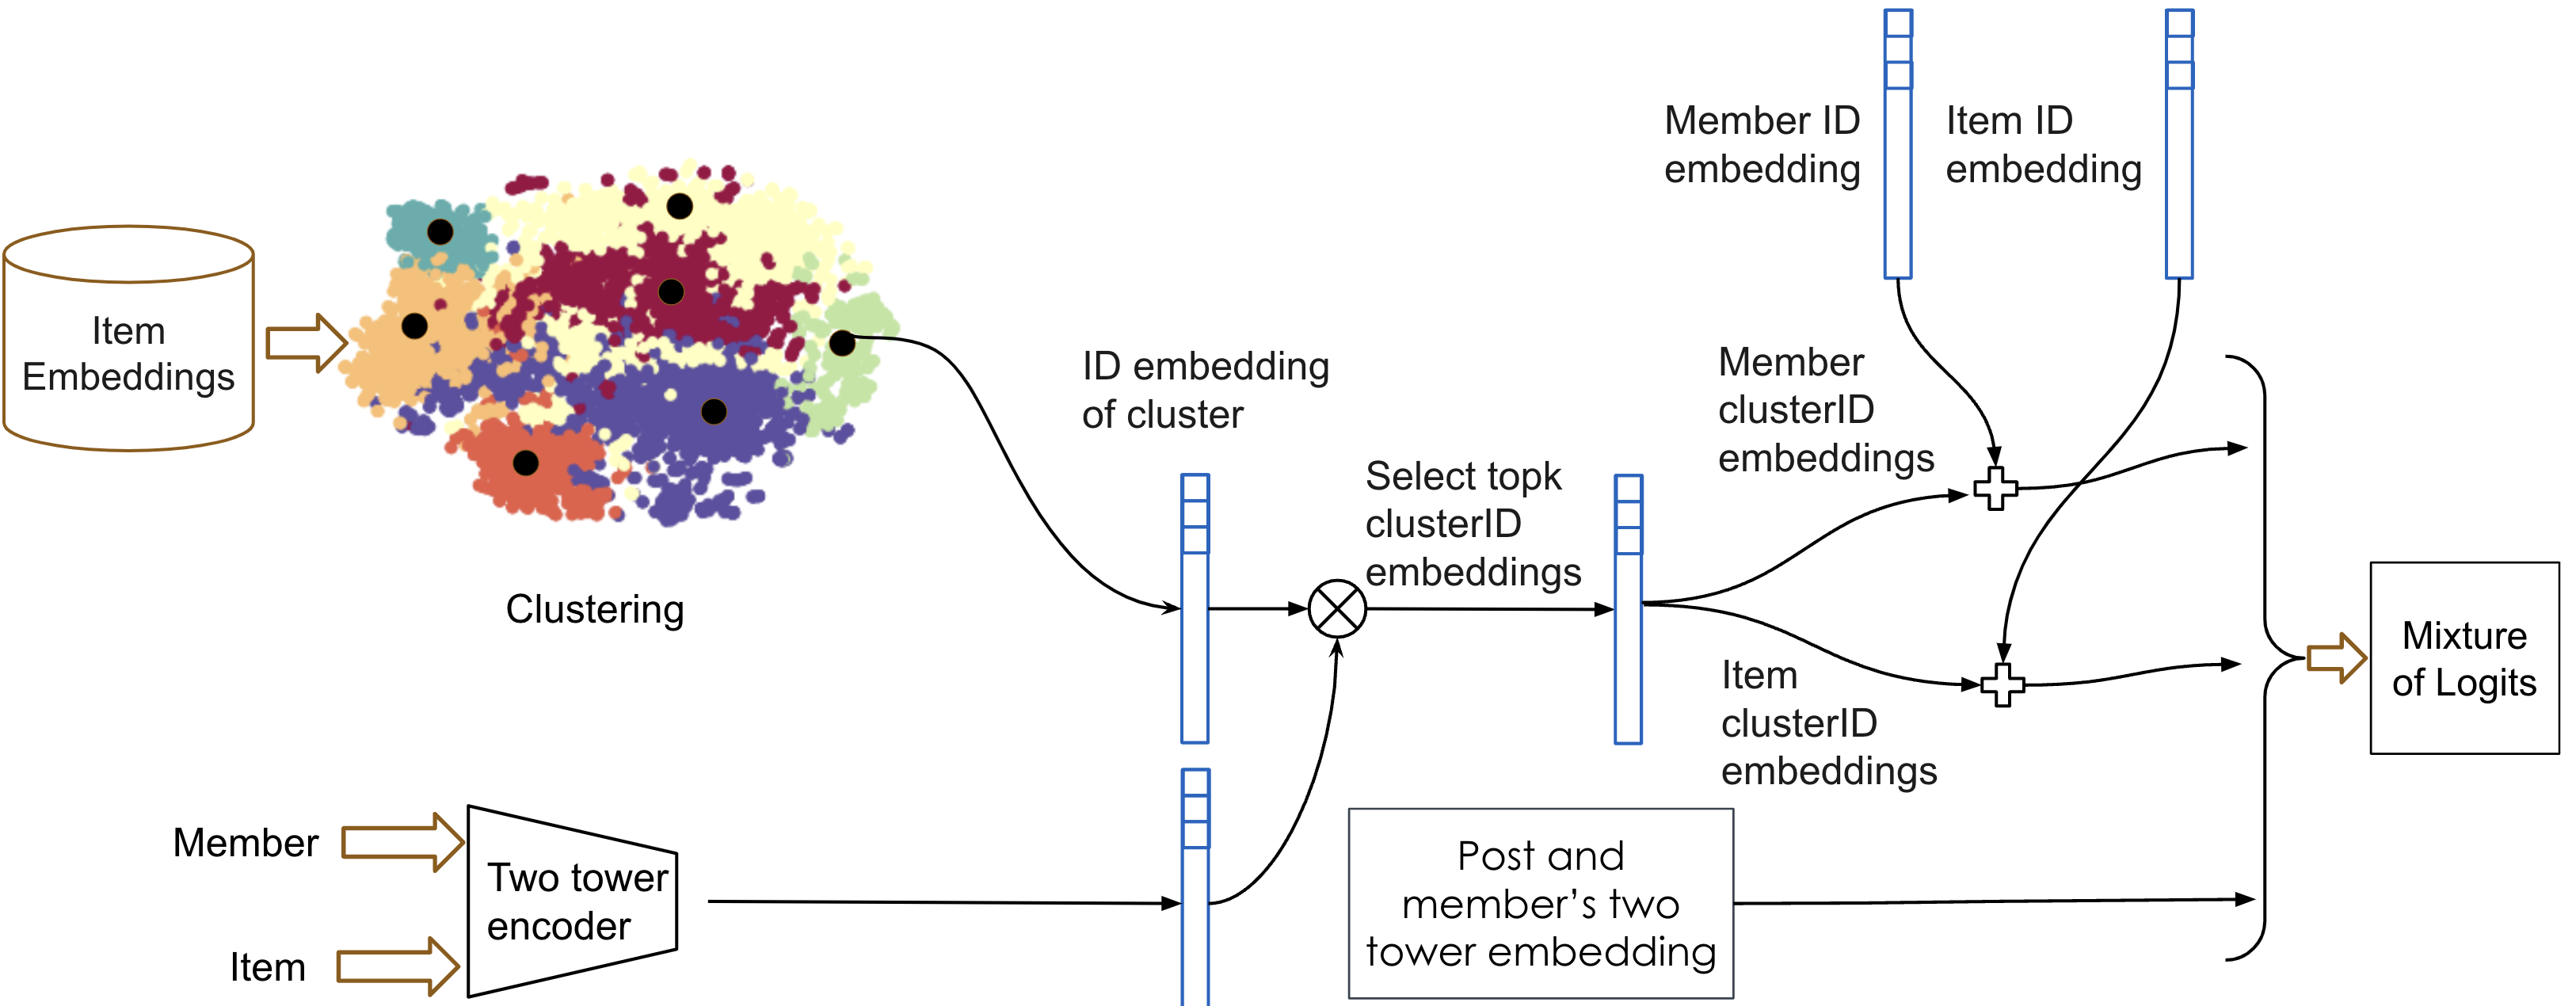
\includegraphics{figures/Cluster_embeddings.png}
%    \end{adjustbox}
%    \caption{Process of applying Residual cluster based ID embeddings for members and posts.}
%    \label{fig:Residual_learning}
% \end{figure}
%
\begin{comment}
\subsection{Model ablation study}
\subsubsection{Effect of components}
Table \ref{table:feature_augmentation} describes the gains from the augmented features when using only cosine similarity in mixture-of-logits. We can see residual embeddings are providing the highest gains. However, some of the gains from these components get cannibalized when we combine all the features together as we can see in Table \ref{table:mix_of_similarities}.

\begin{table}[ht]
% centering
\small % This command makes the text of the table smaller
\begin{tabular}{lcc}
\hline
\textbf{Method}
& \textbf{Hit Rate @ 100} \\\hline 
Baseline (cosine similarity) & 0.00126 \\
k-means++ clusters & 0.0011026 \\
Learnt clusters & 0.00200 \\
Residual id embeddings  & 0.03437274879 \\\hline
\end{tabular}
\caption{Comparison of augmented features}
\label{table:feature_augmentation}
\end{table}

\subsubsection{Effect of similarities}
Table \ref{table:similarity_ablation} describes the gains from the additional similarity functions. We can see that bulk of the gains are being driven by the Hadamard MLP similarity function.

\begin{table}[ht]
% centering
\small % This command makes the text of the table smaller
\begin{tabular}{lcc}
\hline
\textbf{Method}
& \textbf{Hit Rate @ 100} \\\hline 
Baseline (mixture-of-logits with cosine similarity) & 0.034432\\
mixture-of-logits with weighted inner product & 0.03449036299 \\
mixture-of-logits with Hadamard MLP  & 0.03453857363 \\\hline
\end{tabular}
\caption{Comparison of augmented features}
\label{table:similarity_ablation}
\end{table}
\end{comment}

\subsection{A/B test of \systemname}\label{sec:A_b_test}
For our baseline a dot-product EBR is done across all eligible items given member embedding query. We enabled cache on a cloud based storage for online lookup of computed results. This top K is retrieved by mid tier service when an online feed request is received. 
We leveraged this retrieval framework to test RAR based algorithms to understand relevance impact. The baseline for these experiments are full scan dot-product.

\begin{table}[ht]
\small
\vspace{-4pt}
\begin{tabular}{ll}
\hline
\textbf{Metric Name}
& \textbf{Metric Lift} \\\hline 
{Total professional interactions}            & +7\%   \\
{Daily Unique Gold Professional Interactors}  & +3\%   \\
{Feed Update Views With 30+ Secs Dwell}   & +2\%   \\
{Feed Update Viewers With 30+ Secs Dwell} & +5\%   \\
{Skipped Update Rate}                         & -20\% \\\hline
\end{tabular}
\caption{\small {\systemname} A/B test relative metric improvements.}
\label{table:wdotonline}
\vspace{-12pt}
\end{table}

Table~\ref{table:wdotonline} shows the A/B test results from ramp of {\systemname}. \emph{Total professional interactions} are the total amount of high quality interactions in the form of reshares, reposts, comments, message responses, reacts, votes, saves, and long dwells. \emph{Daily Unique Gold Professional Interactors} is the daily moving average of the number of members or companies generating high quality interactions. \emph{Feed Update Views With 30+ Secs Dwell} counts the total number of feed updates viewed with 30+ secs dwell time. \emph{Feed Update Viewers With 30 Plus Secs Dwell} counts the total number of unique members that viewed a feed update for 30+ secs. \emph{Skipped Update Rate} is the ratio of updates that are skipped (viewed for less than 2 seconds) compared to all viewed updates.

\subsection{Model Inference Benchmarking}\label{sec:model_benchmark}
We conducted offline experiments to benchmark the effectiveness of different framework implementations of two KNN variants with ABM on datasets with different pass-rate scenarios. V1 represents KNN with similarity masking, and V2 represents KNN with explicit pre-filtering. Both are implemented in TF and PyTorch with CUDA kernel for attribute matching registered as a custom operator. 
We selected the Job recommendation index for benchmarking due to its variety of filters, providing multi-dimensional performance insights for {\systemname}. The high-pass-rate and low-pass-rate datasets are derived from job search tasks, containing around 15.5 million jobs with 25 thousand queries. The high-pass-rate dataset includes two clauses: geo-location matching and company name reverse matching (mismatched items are returned), with an average of 1.7 million items passing the clauses. The low-pass-rate dataset includes an additional job title exact matching clause, with a maximum pass rate of 1.2 million for single title matching and most queries having only thousands of passed items. Each item and query has one attribute per clause, converted to 64-bit integers before GPU comparison. The embedding dimension is 128, stored as fp16 values. Performance is measured by average latency, p95 latency in milliseconds, and recall label@2000.

\subsubsection{High-Pass-Rate ABM Dataset Benchmarking}\label{sec:high-pass}


\begin{table}[ht]
\centering
\small
\vspace{-4pt}
%\scriptsize 
\begin{tabular}{@{}lccccc@{}}
\hline
\textbf{Method} & \textbf{Batch} & \textbf{\begin{tabular}[c]{@{}c@{}}Avg. Latency\\ (ms/batch)\end{tabular}}

& \textbf{\begin{tabular}[c]{@{}c@{}}P95 Latency\\ (ms/batch)\end{tabular}}

%\textbf{Avg. Latency (ms/batch)}  
%& \textbf{P95 Latency (ms/batch)} 
& \textbf{Recall@2k} \\ \hline
TF-V1              & 1  & 6.3    & 6.9  & 0.688 \\
TF-V2              & 1  &  6.9   & 14.4 & 0.688 \\
PyTorch-V1         & 1  &  4.8   & 4.9 & 0.688 \\
PyTorch-V2         & 1  &  14.6   & 47.8 & 0.688 \\\hline
% CUDA-V2            & 1  &     &  & 0.688 \\
% CUDA-V3-Q400k      & 1  &     &  & 0.685 \\\hline
% PyTorch-V3-Q400k      & 1 &     &  & 0.684\\\hline

TF-V1              & 16 &  34.8   & 36.6  & 0.688 \\
PyTorch-V1         & 16 &   22.8  & 23.1 & 0.688 \\\hline
% CUDA-V2            & 16 &     &  & 0.688 \\
% CUDA-V3-Q400k      & 16 &     &  & 0.685 \\\hline
% PyTorch-V3-Q400k      & 16 &    &  & 0.684 \\\hline
\end{tabular}
\caption{\small Comparison of implementations on high-pass-rate dataset.}
\label{table:high_pass_knn}
\vspace{-18pt}
\end{table}

% \begin{table}[ht]
% \centering
% \scriptsize % This command makes the text of the table smaller
% \begin{tabular}{lccccc}
% \hline
% \textbf{Method} & \textbf{Batch} & \textbf{Avg. Latency (ms)}  & \textbf{P95 Latency (ms)} & \textbf{Recall@2k} \\ \hline
% TF-V1              & 1  &  16.9   & 17.5  & 0.688 \\
% TF-V2              & 1  &  15.9   & 39.1 & 0.688 \\
% PyTorch-V1         & 1  &  12.8   & 13.0 & 0.688 \\
% PyTorch-V2         & 1  &  12.8   & 13.0 & 0.688 \\
% % CUDA-V2            & 1  & 5.1    & 10.5 & 0.688 \\
% % CUDA-V3-Q400k      & 1  & 3.9    & 5.5  & 0.685 \\\hline
% PyTorch-V3-Q400k      & 1 &  10.5   & 11.0 & 0.684\\\hline

% TF-V1              & 16 &  92.0   & 94.0 & 0.688 \\
% PyTorch-V2         & 16 &  57.6   & 57.8 & 0.688 \\\hline
% % CUDA-V2            & 16 &  30.4   & 39.2 & 0.688 \\
% % CUDA-V3-Q400k      & 16 &  27.2   & 30.7 & 0.685 \\\hline
% PyTorch-V3-Q400k      & 16 &  55.5   & 56.0 & 0.684 \\\hline
% \end{tabular}
% \caption{Comparison of different implementations on high-pass-rate dataset on single V100 GPU.}
% \label{table:high_pass_knn}
% \end{table}

From Table~\ref{table:high_pass_knn}, we see that on the high-pass-rate dataset, both TF and PyTorch implementations of V1 (exhaustive search) are faster than V2 (explicit pre-filtering). This is likely due to the native slicing and copying operations in TF and PyTorch, which are especially slow for large matrices, as in V2 with high-pass-rate filters. Benchmarking individual operations revealed that the top-K selection in the latest TF version is slower than in PyTorch, while large-matrix slicing is slower in PyTorch than in TF, leading to performance differences between frameworks. V1's implementation in the high-pass-rate dataset benefits more from the PyTorch implementation with increased batch sizes. Testing the V3 quantized KNN version showed further latency improvements with a trade-off in recall. In this experiment, we used 512-bit quantized embeddings and explored filtering different percentages of items based on quantized embedding similarity before full-precision similarity calculation. The trade-off between latency and recall, correlated with the filter size hyperparameter, is shown in Figure~\ref{fig:high-pass-v3-tradeoff}. By retaining 1\% of items with an additional approximate ranking stage, we achieved around 10\% further latency improvement with nearly parity performance.


\begin{table}[ht]
\centering
\small
\vspace{-4pt}
%\scriptsize % This command makes the text of the table smaller
\begin{tabular}{lcccc}
\hline
\textbf{Method} & \textbf{Batch} & 
\textbf{\begin{tabular}[c]{@{}c@{}}Avg. Latency\\ (ms/batch)\end{tabular}} &

\textbf{\begin{tabular}[c]{@{}c@{}}P95 Latency\\ (ms/batch)\end{tabular}}
%\textbf{Avg. Latency (ms/batch)}  & \textbf{P95 Latency (ms/batch)} 

\\\hline %& \textbf{Recall label@2k} \\ \hline
TF-V2              & 1 & 3.4   & 4.5  \\ % & 100\% \\
PyTorch-V2         & 1 & 1.9  & 2.1  \\\hline % & 100\% \\\hline
% CUDA-V2            & 1 &   &   \\\hline % & 100\% \\\hline
TF-V2              & 16 & 14.2  & 14.8 \\ % 100\% \\
PyTorch-V2         & 16 & 21.4  & 21.9 \\\hline % 100\% \\\hline
% CUDA-V2            & 16 &    &  & 100\% \\\hline
\end{tabular}
\caption{\small Comparison of implementations on low-pass-rate dataset.}
\label{table:low_pass_knn}
\vspace{-16pt}
\end{table}

%From Table~\ref{table:high_pass_knn}, we can see that, on high-pass-rate dataset, the Both TF and PyTorch implementation of V1 exhaustive search is faster than the V2. We attribute this to the fact that the native slicing and copying operations in TF and PyTorch is especially for large matrices, which is the case in the V2 for high-pass-rate filters. Also, via benchmarking different operations individually, we found that the top-K selection operation in the latest TF version is also slower than the PyTorch implementation while the large-matrix slicing operation is slower in PyTorch than TF, leading to the difference in same KNN variant implemented via the two frameworks. Given the benefit of V1 implementation in high-pass-rate dataset, we can gain larger benefits from the PyTorch implementation by increasing the batch size. 

%We also tested the V3 quantized KNN version and saw further latency improvement with a trade-off on the recall. We generate 512 bits quantized embeddings in this experiment and explore different percentage of filtered items based based on the quantize embedding similarity before full-precision similarity calculation. The trade-off between the latency and the recall correlated with the filter size hyperparameter selection is shown in Figure~\ref{fig:high-pass-v3-tradeoff}. By keeping 1\% of items with an extra approximated ranking stage, we could got around 10\% further latency improvement with roughly parity performance.


\begin{figure}
    \centering
    \vspace{-4pt}
    \begin{adjustbox}{max size={\linewidth}{\textheight}}
        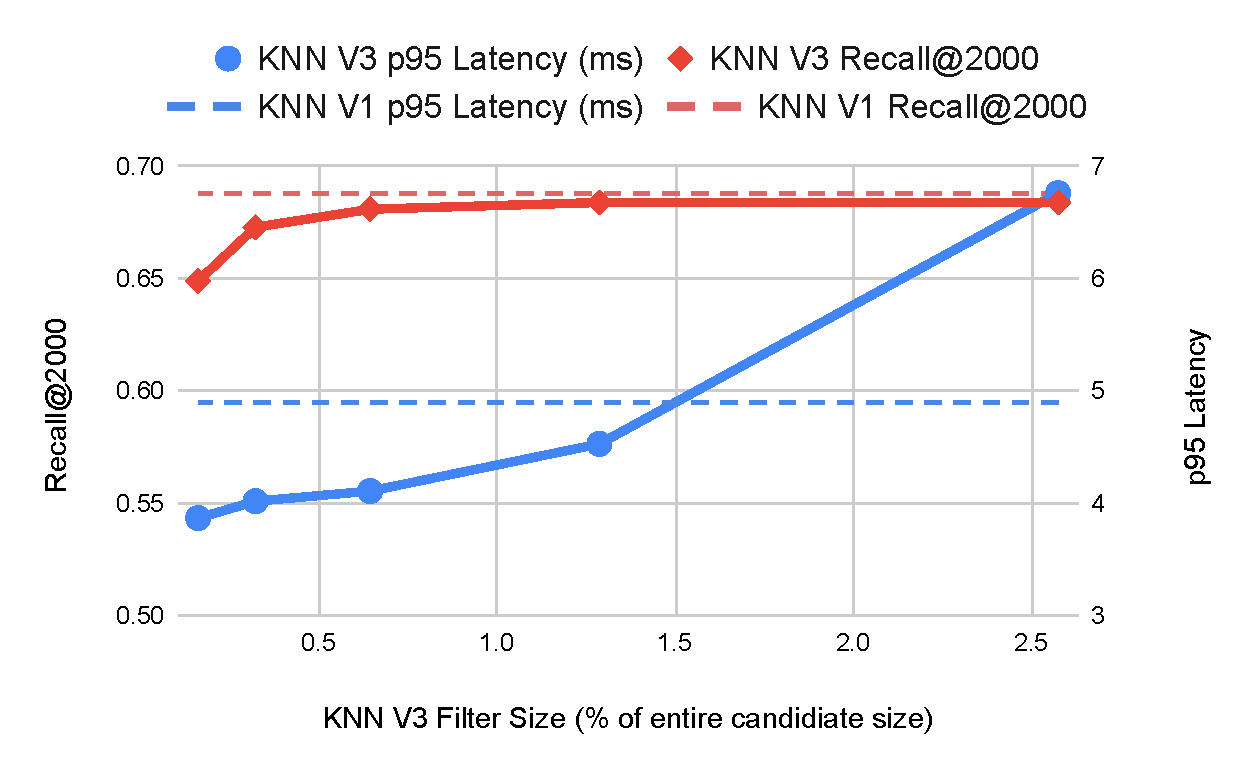
\includegraphics{figures/knn_v3_tradeoff.pdf}
    \end{adjustbox}
    \caption{\small Trade-off of latency and recall correlated with the filter size of V3 quantized KNN with ABM on high-pass-rate dataset.}
    \label{fig:high-pass-v3-tradeoff}
    \vspace{-12pt}
\end{figure}

\subsubsection{Low-Pass-Rate ABM Dataset Benchmarking}\label{sec:low-pass}
%Since V2 version excels in low-pass-rate datasets compared to the other versions (V3 may introduce redundant quantized matrix computation and filtering in this scenario), we compare its performance implemented with TF and PyTorch in Table~\ref{table:low_pass_knn}. For a single query, PyTorch shows an advantage, but TF performs better with larger batch sizes. This is likely due to TF's superior parallel schema for conducting retrievals in parallel. Although queries are fetched in batches, each query has different filters, leading to varied sets and numbers of retrieved items. Therefore, we split the query batch and perform retrieval independently in parallel. Given that V2 is an exhaustive KNN search without liquidity issues, there is no recall drop, and the results are reported here.
As V2 version has the superiority on the low-pass-rate dataset compared to the other two versions (V3 may introduce redundant quantize matrix computation and filtering in the low-pass-rate case), we compare the its performance implemented with TF and PyTorch in Table~\ref{table:low_pass_knn}. One single query, PyTorch still shows its advantage, but TF performs better on larger batch size. We attribute this to the fact the TF has better parallel schema for our case to conduct the retrieval in parallel. Though the queries are fetched in batch, since each query has different filters leading to different sets and number of retrieved items, we split the query batch and conduct the retrieval in parallel for each query independently. Considering that V2 is an exhaustive KNN search without liquidity issue, no recall drop and results are reported here.


\begin{table}[ht]
\centering
\small
\vspace{-4pt}
%\scriptsize % This command makes the text of the table smaller
\begin{tabular}{@{}lccccc@{}}
    \hline
\textbf{Update Per Sec} & \textbf{Batch} & \textbf{QPS} & 
\textbf{\begin{tabular}[c]{@{}c@{}}Avg. Latency\\ (ms/batch)\end{tabular}} &

\textbf{\begin{tabular}[c]{@{}c@{}}P95 Latency\\ (ms/batch)\end{tabular}}
%\textbf{Avg. Latency (ms/batch)}  
%& \textbf{P95 Latency (ms/batch)
\\\hline %& \textbf{Recall label@2k} \\ \hline

0              & 1 & 218 & 4.57  &  4.79 \\ % & 100\% \\
300         & 1 & 215 & 4.64  &  4.93 \\ % & 100\% \\
600         & 1 & 217 & 4.58  &  4.80 \\\hline % & 100\% \\\hline
0              & 5 & 93 & 10.66  &  11.10 \\ % & 100\% \\
300         & 5 & 93 & 10.70  &  11.15 \\ % & 100\% \\\hline
600         & 5 & 93 & 10.70  &  11.16 \\\hline % & 100\% \\\hline

\end{tabular}
\caption{\small Inference latency with concurrent model update.}
\label{table:low_pass_knn}
\vspace{-12pt}
\end{table}

% \begin{table}[ht]
% \centering
% \small % This command makes the text of the table smaller
% \begin{tabular}{lcccc}
% \hline
% \textbf{Method} & \textbf{Batch} & \textbf{Avg. Latency (ms)}  & \textbf{P95 Latency (ms)} \\\hline %& \textbf{Recall label@2k} \\ \hline
% TF-V2              & 1 & 4.0   &  4.7 \\ % & 100\% \\
% PyTorch-V2         & 1 & 2.8   &  3.1 \\\hline % & 100\% \\\hline
% % CUDA-V2            & 1 & 2.5   &  2.6 \\\hline % & 100\% \\\hline
% TF-V2              & 16 &  23.1  & 24.7 & \\ % 100\% \\
% PyTorch-V2         & 16 &  39.2  & 37.2 & \\\hline % 100\% \\\hline
% % CUDA-V2            & 16 &  23.5  & 24.0 & 100\% \\\hline
% \end{tabular}
% \caption{Comparison of different implementations on low-pass-rate dataset on single V100 GPU.}
% \label{table:low_pass_knn}
% \end{table}


% \subsubsection{Stretch Test on Single A100 GPU}
We also conduct a stretch testing on single A100 GPU to measure the capacity of the exhaustive search method on handling large amount of items. For plain KNN with ABM (V1 \& V2) on the high-pass-rate dataset, we are able to handle upto 240 million embeddings with 128 dim and fp16 precision for top-2k selection with single query. For the quantized KNN on an internal notification use case, which we select top-50million members from 1 billion members (64 dimensional embedding saved as fp16) to send relevant notifications, the 1-bit quantized KNN method with 64 bits quantized embedding size can reduce the original 120GB embedding memory to 7.5GB. When processing single query on an A100 GPU, it achieves maximum 21GB high-bandwidth memory with 97.6ms p95 latency.

\subsubsection{Impact of Live Model Update on Inference}\label{sec:low-pass}
We run a benchmark to measure the impact of live model update on the inference latency on a single A100 GPU using our native serving system and bench marking tool. The bench marking tool uses a client for the native serving service and issues requests serially. We use plain KNN model with ABM (V1) and repeat the runs with various concurrent update rates and request batch sizes. We observe no measurable impact on the latency with increased update rate.

